% Options for packages loaded elsewhere
\PassOptionsToPackage{unicode}{hyperref}
\PassOptionsToPackage{hyphens}{url}
%
\documentclass[
]{article}
\usepackage{amsmath,amssymb}
\usepackage{lmodern}
\usepackage{iftex}
\ifPDFTeX
  \usepackage[T1]{fontenc}
  \usepackage[utf8]{inputenc}
  \usepackage{textcomp} % provide euro and other symbols
\else % if luatex or xetex
  \usepackage{unicode-math}
  \defaultfontfeatures{Scale=MatchLowercase}
  \defaultfontfeatures[\rmfamily]{Ligatures=TeX,Scale=1}
\fi
% Use upquote if available, for straight quotes in verbatim environments
\IfFileExists{upquote.sty}{\usepackage{upquote}}{}
\IfFileExists{microtype.sty}{% use microtype if available
  \usepackage[]{microtype}
  \UseMicrotypeSet[protrusion]{basicmath} % disable protrusion for tt fonts
}{}
\makeatletter
\@ifundefined{KOMAClassName}{% if non-KOMA class
  \IfFileExists{parskip.sty}{%
    \usepackage{parskip}
  }{% else
    \setlength{\parindent}{0pt}
    \setlength{\parskip}{6pt plus 2pt minus 1pt}}
}{% if KOMA class
  \KOMAoptions{parskip=half}}
\makeatother
\usepackage{xcolor}
\usepackage[margin =2cm]{geometry}
\usepackage{listings}
\newcommand{\passthrough}[1]{#1}
\lstset{defaultdialect=[5.3]Lua}
\lstset{defaultdialect=[x86masm]Assembler}
\usepackage{longtable,booktabs,array}
\usepackage{calc} % for calculating minipage widths
% Correct order of tables after \paragraph or \subparagraph
\usepackage{etoolbox}
\makeatletter
\patchcmd\longtable{\par}{\if@noskipsec\mbox{}\fi\par}{}{}
\makeatother
% Allow footnotes in longtable head/foot
\IfFileExists{footnotehyper.sty}{\usepackage{footnotehyper}}{\usepackage{footnote}}
\makesavenoteenv{longtable}
\usepackage{graphicx}
\makeatletter
\def\maxwidth{\ifdim\Gin@nat@width>\linewidth\linewidth\else\Gin@nat@width\fi}
\def\maxheight{\ifdim\Gin@nat@height>\textheight\textheight\else\Gin@nat@height\fi}
\makeatother
% Scale images if necessary, so that they will not overflow the page
% margins by default, and it is still possible to overwrite the defaults
% using explicit options in \includegraphics[width, height, ...]{}
\setkeys{Gin}{width=\maxwidth,height=\maxheight,keepaspectratio}
% Set default figure placement to htbp
\makeatletter
\def\fps@figure{htbp}
\makeatother
\setlength{\emergencystretch}{3em} % prevent overfull lines
\providecommand{\tightlist}{%
  \setlength{\itemsep}{0pt}\setlength{\parskip}{0pt}}
\setcounter{secnumdepth}{-\maxdimen} % remove section numbering
\usepackage{titlesec}
\titleformat{\paragraph}
   {\normalfont\bfseries}
   {}
   {0pt}
   {}
\lstset{
  breaklines=TRUE
}

\usepackage[T1]{fontenc}
\usepackage{babel}
\usepackage{geometry}
\usepackage{titling}
\usepackage{blindtext}

\setlength{\droptitle}{-4em}     % Eliminate the default vertical space
\addtolength{\droptitle}{-4pt}   % Only a guess. Use this for adjustment
\pretitle{\begin{center} \vspace{10cm}}
\ifLuaTeX
  \usepackage{selnolig}  % disable illegal ligatures
\fi
\IfFileExists{bookmark.sty}{\usepackage{bookmark}}{\usepackage{hyperref}}
\IfFileExists{xurl.sty}{\usepackage{xurl}}{} % add URL line breaks if available
\urlstyle{same} % disable monospaced font for URLs
\hypersetup{
  pdftitle={Logistic Regression Analysis},
  pdfauthor={B.M Njuguna},
  hidelinks,
  pdfcreator={LaTeX via pandoc}}

\title{\textbf{Logistic Regression Analysis}}
\author{\textbf{B.M Njuguna}}
\date{\textbf{2022-09-27}}

\begin{document}
\maketitle

\newpage 
\tableofcontents
\newpage

\hypertarget{introduction}{%
\section{1.0 Introduction}\label{introduction}}

\textbf{Logistic Regression} is used to predict the category or class of
individuals using one or multiple predictor variables. Logistic
regression estimates the probability of an event occurring, therefore,
since the outcome is probability, the dependent variable is bounded
between 0 and 1. It is used to predict the outcome of a binary (such as
yes or no) based on past values of the data. Logistic regression belongs
to the family of \textbf{Generalized Linear Models (GLM)} which was
built to extend the Linear Regression Model. Logistic Regression is also
known as \emph{binary logistic regression} ,\emph{binomial logistic
regression} or \emph{logit regression}. The model was initially
introduced by Joseph Berkson in 1944. The \emph{response variable} which
I will refer as \(Y\) in this paper, is parametarized by
\(0\space or\space 1\). Traditionally, \(1\) is indicates a
\emph{success} while \(0\) indicates a \emph{failure} or \emph{lack of
success}. \(1\) can also be thought of having a certain characteristic,
condition, requirement or property while \(0\) can be thought of having
certain characteristics or properties. This type of regression is widely
used in epidemiological data analysis. For example, we might have a
research question such as; \emph{what is the relationship between one or
more exposure variable(s) say E to a disease or illness outcome D}. Let
us further take an example of smoking habits and Coronary Heart
Disease(CHD), where the question is to which extent is CHD related with
smoking. Here, \(1\) will represent smoker and \(0\) non smoker for the
case of the independent variable smoking. Also, \(1\) will represent
\emph{diseased or having CHD} and \(0\) will represent \emph{not
diseased or not having CHD} , for the case of the response variable.

Other independent variables such as age, race and sex are known as
\textbf{control variables} (\(C_s\)) . These control variables together
with the binary variables \(E_S\) form a collection of independent
variables which are used to predict the outcome of the response
variable. More generally, as usual, the independent variables are
represented with \(X\) regardless of whether they are \(C_s\) or \(E_s\)
-\emph{Note that the subscript s is used to represent prural or many
variables}. Also, in logistic regression the dependent variable is
always a binary outcome.

It is important to note that logistic regression is based on the
logistic function below;

\[f(z)=\frac{1}{1+e^{-z}}\space\space for\space\space -\infty<z<\infty \]

The graph of this function is shown below;

\begin{lstlisting}[language=R]
> eq = function(z) {
+     1/(1 + exp(-z))
+ }
> library(ggplot2)
> base <- ggplot() + xlim(-5, 5) + ylim(-1, 1)
> base + geom_function(fun = eq, col = "red") + geom_hline(yintercept = c(0, 1), linetype = "dotted") +
+     geom_vline(xintercept = 0, linetype = "dotted")
\end{lstlisting}

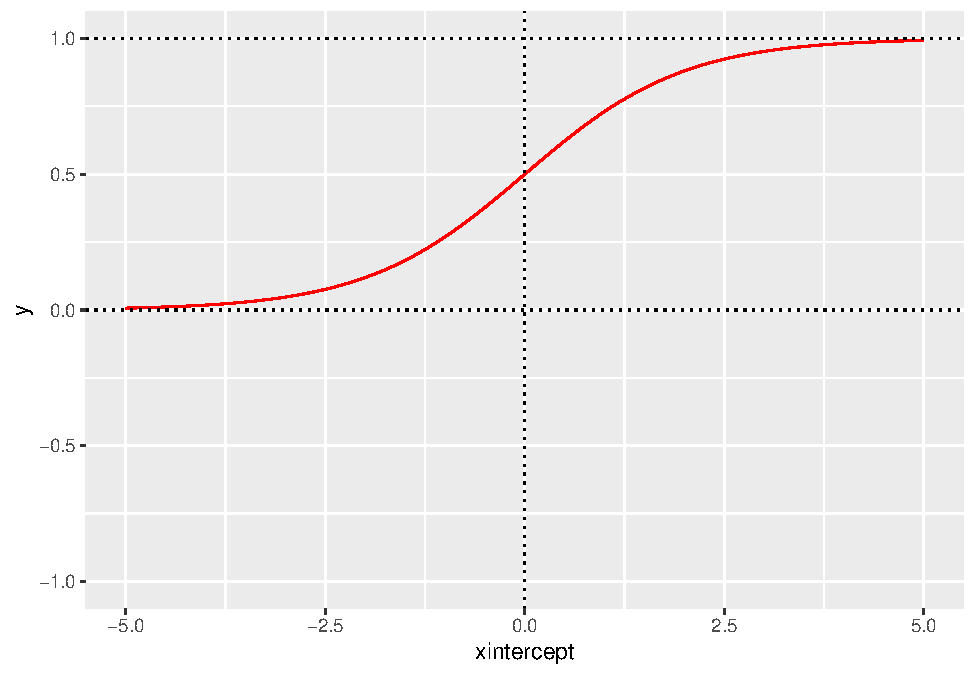
\includegraphics{Logistic-regression_files/figure-latex/unnamed-chunk-1-1.pdf}

Notice that for \(z=-\infty\), then \(f(z)=0\) and for \(z=\infty\),then
\(f(z)=1\). Thus the value of \(f(z)\) ranges from zero to one
regardless of the value of \(z\), which is the primary reason as to why
logistic regression is popular. As mentioned earlier, the response
variable to be predicted is a probability, and as you know probability
ranges from zero to one, hence this model is suitable.

The elongated \textbf{S} shape of the function appeals the
epidemiologists if \(z\) represents an index that combines the
contribution of several risk factors and \(f(z)\) represents the risk
for a given value of \(z\). As in most diseases and risk factors, the
logistic function shows that at low level exposure, the individual's
risk is minimal until it reaches a certain threshold after which the
risk increases rapidly, to a certain threshold also where the risk
remains extremely high.

\hypertarget{the-logistic-model}{%
\section{1.1 The Logistic Model}\label{the-logistic-model}}

To obtain the logistic model, we write \(z\) as a linear sum of
\(x\space\space and \space\space \beta_i\) as follows;

\[z=\beta_0+\beta_1x_1+\beta_2x_2+\dots\beta_nx_n\]

Then, substituting for \(z\) in the logistic function above, we get;

\[f(z)=\frac{1}{(1+e^{-(\beta_0+\sum_{i=1}^n\beta_i x_i)}}\]

Assuming that \(D\) is the disease whose probability is being modeled,
then we denote \(f(z)\) as follows;

\[\mathbb{P}(D|x_1,x_2\dots x_i)=\frac{1}{(1+e^{-(\beta_0+\sum_{i=1}^n\beta_i x_i)}}\]

By multiplication, it can be shown that;

\[\frac{\mathbb{P}(D)}{1-\mathbb{P}(D)}=e^{(\beta_0+\beta_1x1+\dots+\beta_nx_n)}\]

Taking log on both sides we get;
\[\log(\frac{\mathbb{P}(D)}{1-\mathbb{P}(D)})=\beta_0+\beta_1x_1+\dots+\beta_nx_n\]

The quantity \(\log\{\frac{\mathbb{P}(D)}{1-\mathbb{P}(D)}\}\) is known
as \textbf{log-odd} or the \textbf{logit}. The \textbf{odd} refer to the
likelihood of an event occurring. It can also be seen as the ratio of
``success'' to ``non-success''.

\hypertarget{simple-logistic-model}{%
\subsection{1.1.1 Simple Logistic Model}\label{simple-logistic-model}}

The simple logistic model is used to estimate the probability of class
membership based on one predictor or independent variable. The model is
written as;

\[\mathbb{P}(D|x_1)=\frac{1}{(1+e^{-(\beta_o+\beta_1x_1)})}\]

To understand this type of regression, let us use an example where let
the disease of interest \(D\) be \(CHD\) or Coronary Heart Disease. We
wish to find out whether a certain gender increases the risk of
contracting CHD. I am going to use a data set publicly available on
\emph{Kaggle}. The data set is from a study of cardiovascular study on
residents of the town of Framingham, Massachusetts, which recorded
whether the persons in the study contracted CHD.

\begin{lstlisting}[language=R]
> ## Importing the data
> setwd("D:/Documents/R-Studio Programms/Regression/Logistic Regression")
> library(readxl)
> CHD <- read_excel("CHD.xlsx")
> 
> head(CHD)
\end{lstlisting}

\begin{lstlisting}
## # A tibble: 6 x 10
##   Gender   age currentSmoker cigsPerDay   Hyp  Chol   BMI heartRate glucose
##    <dbl> <dbl>         <dbl>      <dbl> <dbl> <dbl> <dbl>     <dbl>   <dbl>
## 1      1    39             0          0     0   195  27.0        80      77
## 2      0    46             0          0     0   250  28.7        95      76
## 3      1    48             1         20     0   245  25.3        75      70
## 4      0    61             1         30     1   225  28.6        65     103
## 5      0    46             1         23     0   285  23.1        85      85
## 6      0    43             0          0     1   228  30.3        77      99
## # ... with 1 more variable: CHD <dbl>
\end{lstlisting}

\begin{lstlisting}[language=R]
> ## Data Preparation
> CHD$Gender <- factor(CHD$Gender, levels = c(0, 1), labels = c("Female", "Male"))
> CHD$currentSmoker <- factor(CHD$currentSmoker, levels = c(0, 1), labels = c("No",
+     "Yes"))
> CHD$Hyp <- factor(CHD$Hyp, levels = c(0, 1), labels = c("No", "Yes"))
> 
> CHD$CHD <- factor(CHD$CHD, levels = c(0, 1), labels = c("No", "Yes"))
\end{lstlisting}

We however need to divide our data into two parts, one for training the
model \emph{commonly known as training data} and the other for testing
our model , known as \emph{test data}. In most cases, we use \(70\%\) of
the total data as the training data and the rest \(30\%\) as the testing
data. This is shown below;

\begin{lstlisting}[language=R]
> trainningdata <- CHD[c(1:2660), ]
> testdataCHD <- CHD[c(2661:3800), ]
\end{lstlisting}

Hence from the training data we can build our model as;

\begin{lstlisting}[language=R]
> model1 <- glm(CHD ~ Gender, family = binomial, data = trainningdata)
> summary(model1)
\end{lstlisting}

\begin{lstlisting}
## 
## Call:
## glm(formula = CHD ~ Gender, family = binomial, data = trainningdata)
## 
## Deviance Residuals: 
##     Min       1Q   Median       3Q      Max  
## -0.6519  -0.6519  -0.5184  -0.5184   2.0364  
## 
## Coefficients:
##             Estimate Std. Error z value Pr(>|z|)    
## (Intercept)  -1.9390     0.0780  -24.86  < 2e-16 ***
## GenderMale    0.4982     0.1078    4.62 3.84e-06 ***
## ---
## Signif. codes:  0 '***' 0.001 '**' 0.01 '*' 0.05 '.' 0.1 ' ' 1
## 
## (Dispersion parameter for binomial family taken to be 1)
## 
##     Null deviance: 2290.0  on 2659  degrees of freedom
## Residual deviance: 2268.6  on 2658  degrees of freedom
## AIC: 2272.6
## 
## Number of Fisher Scoring iterations: 4
\end{lstlisting}

In logistic model, a negative intercept (\(\beta_0\)) implies that the
probability of having the disease or the outcome is below 0.5. A
positive intercept implies that the probability of having the disease or
the outcome is greater than 0.5, while an intercept equal to zero
implies that the probability is approximately equal to 0.5.

From the output above, our model can be written as;

\[\mathbb{P}(CHD|gender)=\frac{1}{(1+e^{-(1.939+0.498gender)})}\]

The odds of CHD infection given that you are a male is 0.191 that if
contracting CHD given that you are a female, as shown below

\[\mathbb{P}(CHD|gender)=\frac{1}{(1+e^{-(-1.939+0.498*1)})}=0.191\]

And the odds of CHD infection given that you are a female is 1.226 that
of CHD infection given that you are male, as shown below;

\[\mathbb{P}(CHD|gender)=\frac{1}{(1+e^{-(1.951+0.492*0)})}=0.126\]

From the above calculations we can conclude that the risk of having CHD
is higher for males than for females. Then if we divide the predicted
risk of males by the predicted risk of females as shown below, we obtain
the \textbf{risk ratio estimate} \(\hat{RR}\).

\[\frac{\mathbb{P}(CHD|male)}{\mathbb{P}(CHD|female)}=\frac{0.191}{0.126}=1.516\]

Finally, we use the test data to predict the probabilities of the given
predictor variables. In R, we use the \textbf{predict.glm} function as
follows;

\begin{lstlisting}[language=R]
> predictmodel1 <- predict.glm(model1, testdataCHD, type = "response")
\end{lstlisting}

The summary of the probabilities is as follows;

\begin{lstlisting}[language=R]
> MODEL1PREDICT = data.frame(testdataCHD$Gender, predictmodel1)
> 
> colnames(MODEL1PREDICT) <- c("Gender", "Predicted Probabilities")
> 
> knitr::kable(MODEL1PREDICT[c(1, 2), ], row.names = FALSE)
\end{lstlisting}

\begin{longtable}[]{@{}lr@{}}
\toprule()
Gender & Predicted Probabilities \\
\midrule()
\endhead
Male & 0.1914163 \\
Female & 0.1257525 \\
\bottomrule()
\end{longtable}

Thus, the probability of contracting CHD given that the gender is Male
is 0.191, while the probability of contracting CHD given that the Gender
is female is 0.125.

The \textbf{null deviance} above is a concept in generalized linear
models that measures the fitted generalized model against a perfect
model known as the \textbf{saturated model}. It is a generalization of
the total sums of squares in a linear model. The null deviance shows how
well the model predicts the response variable with the intercept only.
The smaller the Null Deviance, the better the model.

The \textbf{residual deviance} shows how well a model can predict the
response variable with more than -say \(p\)- predictors. To determine
the usefulness of the model we can calculate a \(\chi^2\) statistic with
\(p\) (number of predictor variables) degrees of freedom as follows;
Note that, the lower the value of residual deviance, the better the
model (Obviously)

\[\chi^2_{(p)}=Null\space deviance\space -\space Residual\space deviance\]

After which we find the p-value associated with the statistic, if it is
less than \(\alpha=0.05\) (for our case), then the model is useful or
significant. We only have one predictor variable, thus the degrees of
freedom = 1.

\[\chi^2_{(1)}= 2290.0-2268.6=21.4\]

\begin{lstlisting}[language=R]
> pchisq(q = 21.4, df = 1, lower.tail = F)
\end{lstlisting}

\begin{lstlisting}
## [1] 3.727712e-06
\end{lstlisting}

Thus since the p-value is less than \(\alpha\), our model is useful.

\hypertarget{multiple-logistic-regression}{%
\subsection{1.1.2 Multiple Logistic
Regression}\label{multiple-logistic-regression}}

The procedure for multiple logistic regression is the same as for the
simple logistic regression. A multiple logistic regression is logistic
regression where more than one predictor variables are used to predict
the response variable. For example, we may wish to know the effect of
age, hypertension, gender, heart rate, smoking habit, BMI level,
cholesterol levels and glucose levels on contracting CHD. In r, we build
a multiple logistic model as follows;

\begin{lstlisting}[language=R]
> model2 <- glm(CHD ~ Gender + age + heartRate + cigsPerDay + Hyp + glucose + Chol +
+     BMI, family = binomial, data = trainningdata)
> summary(model2)
\end{lstlisting}

\begin{lstlisting}
## 
## Call:
## glm(formula = CHD ~ Gender + age + heartRate + cigsPerDay + Hyp + 
##     glucose + Chol + BMI, family = binomial, data = trainningdata)
## 
## Deviance Residuals: 
##     Min       1Q   Median       3Q      Max  
## -1.7690  -0.6136  -0.4318  -0.2897   2.7552  
## 
## Coefficients:
##              Estimate Std. Error z value Pr(>|z|)    
## (Intercept) -7.990591   0.696568 -11.471  < 2e-16 ***
## GenderMale   0.431356   0.125001   3.451 0.000559 ***
## age          0.068937   0.007350   9.379  < 2e-16 ***
## heartRate   -0.003019   0.004912  -0.615 0.538825    
## cigsPerDay   0.024272   0.004907   4.947 7.54e-07 ***
## HypYes       0.580501   0.122945   4.722 2.34e-06 ***
## glucose      0.010452   0.002166   4.826 1.39e-06 ***
## Chol         0.002955   0.001282   2.305 0.021153 *  
## BMI          0.027174   0.013935   1.950 0.051166 .  
## ---
## Signif. codes:  0 '***' 0.001 '**' 0.01 '*' 0.05 '.' 0.1 ' ' 1
## 
## (Dispersion parameter for binomial family taken to be 1)
## 
##     Null deviance: 2290.0  on 2659  degrees of freedom
## Residual deviance: 2038.6  on 2651  degrees of freedom
## AIC: 2056.6
## 
## Number of Fisher Scoring iterations: 5
\end{lstlisting}

From the output above, we can see that most predictor variables are
significant at \(1\%\) level of significance. However, the predictor
variables named heartRate is not significant and should be eliminated to
increase the accuracy of the model. This elimination can be
automatically using statistical techniques, including \textbf{step-wise
regression} and \textbf{penalized regression}.

\begin{lstlisting}[language=R]
> model3 <- glm(CHD ~ Gender + age + cigsPerDay + Hyp + glucose + Chol + BMI, family = binomial,
+     data = trainningdata)
> summary(model3)
\end{lstlisting}

\begin{lstlisting}
## 
## Call:
## glm(formula = CHD ~ Gender + age + cigsPerDay + Hyp + glucose + 
##     Chol + BMI, family = binomial, data = trainningdata)
## 
## Deviance Residuals: 
##     Min       1Q   Median       3Q      Max  
## -1.7700  -0.6121  -0.4326  -0.2887   2.7613  
## 
## Coefficients:
##              Estimate Std. Error z value Pr(>|z|)    
## (Intercept) -8.187185   0.619814 -13.209  < 2e-16 ***
## GenderMale   0.440725   0.124069   3.552 0.000382 ***
## age          0.069116   0.007343   9.413  < 2e-16 ***
## cigsPerDay   0.023888   0.004866   4.909 9.16e-07 ***
## HypYes       0.571101   0.121945   4.683 2.82e-06 ***
## glucose      0.010338   0.002156   4.794 1.63e-06 ***
## Chol         0.002907   0.001279   2.273 0.023051 *  
## BMI          0.026538   0.013886   1.911 0.055989 .  
## ---
## Signif. codes:  0 '***' 0.001 '**' 0.01 '*' 0.05 '.' 0.1 ' ' 1
## 
## (Dispersion parameter for binomial family taken to be 1)
## 
##     Null deviance: 2290.0  on 2659  degrees of freedom
## Residual deviance: 2038.9  on 2652  degrees of freedom
## AIC: 2054.9
## 
## Number of Fisher Scoring iterations: 5
\end{lstlisting}

Thus our model can be written as;

\[\mathbb{P}(CHD|gender,\dots)=\frac{1}{(1+e^{-(-7.537+0.451Gender+0.069Age+0.023CigsPerDay+0.632Hyp+0.011glucose+0.003Cholestrol+0.027BMI)})}\]

From the output above, we see that all the \(\beta\) coefficients of
predictor variables are positive which implies that if any of the
predictor variables is increased, the probability of having CHD
increases (This applies for the control predictor variables) We can also
calculate the odds ratio by taking the exponential of the predictor
variables. For example, the \(\beta\) coefficient for glucose is
\(0.011\) which implies that a one unit increase in glucose will
increase the odds of having CHD by \(e^{0.011}=1.011\) times. Number of
iterations is just a measure of how long it took to fit your model and
you can safely ignore it.

The predicted probabilities are as follows;

\begin{lstlisting}[language=R]
> model3predict <- predict.glm(model3, testdataCHD, type = "response")
> 
> TESTmodel3 = data.frame(testdataCHD[, c(1, 2, 4, 5, 6, 7, 8, 9)], model3predict)
> colnames(TESTmodel3) <- c("Gender", "Age", "CigsPerDay", "Hyp", "Chol", "BMI", "HeartRate",
+     "Glucose", "Predicted Probabilites")
> knitr::kable(TESTmodel3[c(1:8), c(1, 2, 3, 4, 5, 6, 7, 8, 9)], row.names = FALSE)
\end{lstlisting}

\begin{longtable}[]{@{}
  >{\raggedright\arraybackslash}p{(\columnwidth - 16\tabcolsep) * \real{0.0897}}
  >{\raggedleft\arraybackslash}p{(\columnwidth - 16\tabcolsep) * \real{0.0513}}
  >{\raggedleft\arraybackslash}p{(\columnwidth - 16\tabcolsep) * \real{0.1410}}
  >{\raggedright\arraybackslash}p{(\columnwidth - 16\tabcolsep) * \real{0.0513}}
  >{\raggedleft\arraybackslash}p{(\columnwidth - 16\tabcolsep) * \real{0.0641}}
  >{\raggedleft\arraybackslash}p{(\columnwidth - 16\tabcolsep) * \real{0.0769}}
  >{\raggedleft\arraybackslash}p{(\columnwidth - 16\tabcolsep) * \real{0.1282}}
  >{\raggedleft\arraybackslash}p{(\columnwidth - 16\tabcolsep) * \real{0.1026}}
  >{\raggedleft\arraybackslash}p{(\columnwidth - 16\tabcolsep) * \real{0.2949}}@{}}
\toprule()
\begin{minipage}[b]{\linewidth}\raggedright
Gender
\end{minipage} & \begin{minipage}[b]{\linewidth}\raggedleft
Age
\end{minipage} & \begin{minipage}[b]{\linewidth}\raggedleft
CigsPerDay
\end{minipage} & \begin{minipage}[b]{\linewidth}\raggedright
Hyp
\end{minipage} & \begin{minipage}[b]{\linewidth}\raggedleft
Chol
\end{minipage} & \begin{minipage}[b]{\linewidth}\raggedleft
BMI
\end{minipage} & \begin{minipage}[b]{\linewidth}\raggedleft
HeartRate
\end{minipage} & \begin{minipage}[b]{\linewidth}\raggedleft
Glucose
\end{minipage} & \begin{minipage}[b]{\linewidth}\raggedleft
Predicted Probabilites
\end{minipage} \\
\midrule()
\endhead
Male & 55 & 20 & No & 280 & 29.86 & 80 & 75 & 0.2524674 \\
Female & 61 & 0 & Yes & 270 & 29.87 & 80 & 76 & 0.2617960 \\
Male & 38 & 20 & No & 220 & 24.46 & 77 & 74 & 0.0698790 \\
Male & 36 & 20 & No & 252 & 25.23 & 75 & 63 & 0.0613970 \\
Male & 50 & 30 & No & 225 & 29.38 & 79 & 106 & 0.2603100 \\
Male & 42 & 20 & No & 234 & 28.09 & 70 & 70 & 0.0982871 \\
Female & 45 & 0 & Yes & 258 & 23.46 & 85 & 90 & 0.0995018 \\
Female & 48 & 9 & No & 280 & 25.50 & 85 & 79 & 0.0872923 \\
\bottomrule()
\end{longtable}

Thus from the output above, we can get the probabilities that we are
interested in. For instance, the probability that a Male aged 55 years,
smokes 20 cigarettes per day, has no hypertension, cholesterol level is
280, BMI 29.86, Heart Rate 80 and glucose level is 75 contracts CHD is
0.252. You can, therefore, read the desired probabilities.

Note that, we only estimate the Risk Ratio using the logistic regression
if a follow up study was conducted. However, in the case of
Cross-sectional and case control study, we cannot use the logistic
regression to estimate the individual risks but only the odds ratio. In
follow-up study, it is commonly preferred to estimate the Risk Ratio
rather than the Odds Ratio.

\newpage

\hypertarget{multinomial-logistic-regression}{%
\section{2.0 Multinomial Logistic
Regression}\label{multinomial-logistic-regression}}

A \textbf{Multinomial Logistic Regression} is an extension of the
logistic regression which is used when the outcome involves more than
two classes. It allows for more than two categories of the dependent or
the independent variable. Multinomial logistic regression is often
considered an attractive analysis because it does not assume normality,
linearity or homoscedasticity. However, it does have an assumption of
independence of choices in the dependent variable which states that the
choice of or membership in one category is not related to the choice or
membership of another category(IIA). This assumption can be tested using
the \textbf{Hausman-McFadden test}, in r, we use the function
\textbf{hmftest}, from \textbf{mlogit} package. Given that the
categorical response variable \(Y\) has more than two possible levels,
namely \({1,\dots,J}\) and further given that we have
\(X_1,X_2,\dots,X_P\), then the multiple logistic regression models the
probability of each level \(j\) of \(Y\), by;

\[p_J(\mathbf{x}):=\mathbb{P}(Y=j|X_1=x_p,\dots,X_p=x_p)=\frac{1}{(1+\sum_{\ell=1}^{J-1}e^{(\beta_{0\ell}+\beta_{1\ell}X_1+\dots+\beta_{p\ell}X_p)}}\]

The multinomial regression has an interesting interpretation of logistic
regression. For example taking the quotients;

\[\frac{p_j(\mathbf{x})}{p_J(\mathbf{x})}= e^{\beta_{0j}+\beta_{1j}X_1+\dots+\beta_{pj}X_p}\space for\space j=1,\dots,J-1\]

Then taking logarithms on both sides we get;

\[\log{(\frac{p_j(\mathbf{x})}{p_J(\mathbf{x})})}=\beta_{0j}+\beta_{1j}X_1+\dots+\beta_{pj}X_p\]

Thus, if the probabilities on LHS added to one, we would have gotten a
log-odds and hence the logistic regression for \(Y\), which is not the
case. Therefore, due to this effect, we have the \emph{ratios} or the
\emph{log-ratios} of the non-complimentary probabilities. Further,
\(e^{\beta_{0j}}\) is the ratio between \(p_j(\mathbf{0})\) and
\(p_J(\mathbf{0})\), representing the probabilities of \(Y=j\) when
\(X_1=X_2=\dots=X_p=0\).\footnote{Note that the multinomial regression
  is like a set of \(J-1\) independent logistic regressions for the
  probability of \(Y=j\) versus the probability of reference \(Y=J\)}
Note the following;

\begin{enumerate}
\def\labelenumi{\arabic{enumi}.}
\item
  If \(e^{\beta_{0j}}>1\) and \(\beta_{0j}>0\), then the \(Y=j\) is more
  likely than \(Y=J\)
\item
  However, if \(e^{\beta_{0j}}<1\) and \(\beta_{0j}<0\), then \(Y=j\) is
  less likely than \(Y=J\)
\item
  \(e^{\beta_{\ell j}}\) is the \textbf{multiplicative} increment of the
  ratio between \(p_j(\mathbf{x})\) and \(p_J(\mathbf{x})\) for an
  increment in one unit of \(X_\ell=x_\ell\), provided that the
  remaining variables; \(X_1,\dots,X_{\ell-1},X_{\ell+1},\dots,X_p\) do
  not change.
\item
  If \(e^{\beta_{\ell j}}>1\) and equivalently, \(\beta_{\ell j}>0\),
  then \(Y=j\) becomes more likely than \(Y=J\) for each increment in
  \(X_j\).
\item
  if \(e^{\beta_{\ell j}}<1\) and \(\beta_{\ell j}<00\), then \(Y=j\)
  becomes less likely than \(Y=J\) for each increment in \(X_j\).
\end{enumerate}

\hypertarget{examples-of-multinomial-logistic-regression}{%
\subsection{2.1 Examples of Multinomial Logistic
Regression}\label{examples-of-multinomial-logistic-regression}}

\begin{enumerate}
\def\labelenumi{\arabic{enumi}.}
\item
  People's occupation choices might be influenced by their parents'
  occupation and their own educational level. We can model or study the
  relationship between one's occupation, educational level and the
  father's or mother's occupation. The outcome or the response variable
  will be the occupation choices which consists of occupational
  categories.
\item
  A biologist may be interested in the food choices an alligator makes.
  Adult alligators might have different choices from younger ones. Here,
  the response variable will be the food choices while the predictor
  variables can be the size of alligators (which is continuous) and
  other environmental factors.
\item
  High school students makes a program choice among general program,
  vocational program and academic program. Their choice might be modeled
  based on their writing score and social economic status.
\end{enumerate}

In r, there are various packages with inbuilt functions for building a
multinomial logistic regression, but am going to use the \textbf{nnet
package}. Let's us model the student program choice based on their
writing score and social economic status. I'm first going to download
the data set known as \textbf{hsbdemo} from
\href{https://stats.idre.ucla.edu}{stats idre website}

\begin{lstlisting}[language=R]
> require(foreign)
> require(nnet)
> require(ggplot2)
> require(reshape2)
> 
> ## downloading the data
> Student <- read.dta("https://stats.idre.ucla.edu/stat/data/hsbdemo.dta")
> 
> ## A glimpse of the first few rows of the data
> head(Student)
\end{lstlisting}

\begin{lstlisting}
##    id female    ses schtyp     prog read write math science socst       honors
## 1  45 female    low public vocation   34    35   41      29    26 not enrolled
## 2 108   male middle public  general   34    33   41      36    36 not enrolled
## 3  15   male   high public vocation   39    39   44      26    42 not enrolled
## 4  67   male    low public vocation   37    37   42      33    32 not enrolled
## 5 153   male middle public vocation   39    31   40      39    51 not enrolled
## 6  51 female   high public  general   42    36   42      31    39 not enrolled
##   awards cid
## 1      0   1
## 2      0   1
## 3      0   1
## 4      0   1
## 5      0   1
## 6      0   1
\end{lstlisting}

The response variable will be the program -named prog in the data set-
while the predictor variables will be social economic status -named ses-
which is a three-level categorical variable, writing score -named
write-a continuous variable.

First, we need to choose our level of outcome that we wish to use as our
baseline and then specify this with \textbf{relevel} function.

\begin{lstlisting}[language=R]
> Student$prog2 <- relevel(Student$prog, ref = "academic")
\end{lstlisting}

After specifying our baseline level of outcome, We can now use the
function \textbf{multinom} from the \textbf{nnet} package to build the
model.

\begin{lstlisting}[language=R]
> mlt <- multinom(prog2 ~ ses + write, data = Student)
\end{lstlisting}

\begin{lstlisting}
## # weights:  15 (8 variable)
## initial  value 219.722458 
## iter  10 value 179.982880
## final  value 179.981726 
## converged
\end{lstlisting}

\begin{lstlisting}[language=R]
> summary(mlt)
\end{lstlisting}

\begin{lstlisting}
## Call:
## multinom(formula = prog2 ~ ses + write, data = Student)
## 
## Coefficients:
##          (Intercept)  sesmiddle    seshigh      write
## general     2.852198 -0.5332810 -1.1628226 -0.0579287
## vocation    5.218260  0.2913859 -0.9826649 -0.1136037
## 
## Std. Errors:
##          (Intercept) sesmiddle   seshigh      write
## general     1.166441 0.4437323 0.5142196 0.02141097
## vocation    1.163552 0.4763739 0.5955665 0.02221996
## 
## Residual Deviance: 359.9635 
## AIC: 375.9635
\end{lstlisting}

The \emph{multinom} function, does not automatically calculate the
p-values, hence we will do it manually as follows;

\begin{lstlisting}[language=R]
> z <- summary(mlt)$coefficients/summary(mlt)$standard.errors
> z
\end{lstlisting}

\begin{lstlisting}
##          (Intercept)  sesmiddle   seshigh     write
## general     2.445214 -1.2018081 -2.261334 -2.705562
## vocation    4.484769  0.6116747 -1.649967 -5.112689
\end{lstlisting}

We can then proceed to calculate the 2-tailed z-test

\begin{lstlisting}[language=R]
> p <- (1 - pnorm(abs(z), 0, 1)) * 2
> p
\end{lstlisting}

\begin{lstlisting}
##           (Intercept) sesmiddle    seshigh        write
## general  0.0144766100 0.2294379 0.02373856 6.818902e-03
## vocation 0.0000072993 0.5407530 0.09894976 3.176045e-07
\end{lstlisting}

\hypertarget{interpretation-of-the-output}{%
\subsubsection{2.1.1 Interpretation of the
output}\label{interpretation-of-the-output}}

The model summary output has a block of coefficients and a block of
standard errors. Focusing on the block of coefficients, each row
contains a model equation. The first row compares the general program to
our baseline academic program while the second row compares the vocation
programs to academic program. Let the coefficients from the first row be
\(\hat{\beta_1}\) and further let coefficients from the second row be
\(\hat{\beta_2}\), then we can write our model as;

\[\ln(\frac{\mathbb{P}(Program=general)}{\mathbb{P}(Program=academic)})=\hat{\beta_{10}}+\hat{\beta_{11}}(ses=middle)+\hat{\beta_{12}}(ses=high)+\hat{\beta_{13}}write\]

\[\ln(\frac{\mathbb{P}(Program=general)}{\mathbb{P}(Program=academic)})=2.852-0.533(ses=middle)-1.163(ses=high)-0.058write\]

This can be interpreted as:

\begin{itemize}
\item
  A one unit increase in write leads to 0.058 decrease in the log odds
  of being in general program versus academic program.
\item
  The log odds of being in general program vs academic program decreases
  by an average of 1.163 if the student has a high social economic
  status.Or, a high class social economic status student is less likely
  to be in the general program than to be in the academic program
\item
  The log odds of being in general program vs academic program decreases
  by 0.533 if the student has a middle social economic status. Or, a
  middle class social economic status student is less likely to be in
  the general program than to be in the academic program (although not
  significant).
\item
  Since our \(\hat{\beta_{10}}>0\), then, a student is more likely to be
  in the general program than to be in the academic program, in the
  absence of other predictor variables.
\end{itemize}

Now let the coefficients from the second row be \(\hat{\beta_2}\), then
we can write the model as;

\[\ln(\frac{\mathbb{P}(Program=vocation)}{\mathbb{P}(Program=academic)})=\hat{\beta_{20}}+\hat{\beta_{21}}(ses=middle)+\hat{\beta_{22}}(ses=high)+\hat{\beta_{23}}write\]

\[\ln(\frac{\mathbb{P}(Program=vocation)}{\mathbb{P}(Program=academic)})=5.219+0/291(ses=middle)-0.983(ses=high)-0.114write\]

This can be interpreted as;

\begin{itemize}
\item
  A one unit increase in write leads to 0.114 decrease in the log odds
  of being in vocation program versus academic program.
\item
  The log odds of being in vocation program vs academic program
  decreases by 0.983 if the student has a high class social economic
  status. Or, a high class social economic status student is less likely
  to be in the vocation program than to be in the academic program.
\item
  The log odds of being in vocation program vs academic program
  increases by 0.291 if the student has a middle social economic status.
  Or, a middle class social economic status student is more likely to be
  in the vocation program than to be in the academic program (although
  not statistically significant looking at its p-value).
\item
  Since our \(\hat{\beta_{20}}>0\), then, a student is more likely to be
  in the vocation program than to be in the academic program, in the
  absence of other predictor variables.
\end{itemize}

Then the ratio of the probability of choosing one variable outcome over
another is called the relative risk. We obtain it by exponentiation of
the Right Hand Side of the model.

\begin{lstlisting}[language=R]
> exp(coef(mlt))
\end{lstlisting}

\begin{lstlisting}
##          (Intercept) sesmiddle   seshigh     write
## general     17.32582 0.5866769 0.3126026 0.9437172
## vocation   184.61262 1.3382809 0.3743123 0.8926116
\end{lstlisting}

\hypertarget{assumptions-of-the-multinomial-logistic-regression}{%
\subsubsection{2.1.2 Assumptions of the Multinomial Logistic
Regression}\label{assumptions-of-the-multinomial-logistic-regression}}

\begin{enumerate}
\def\labelenumi{\arabic{enumi}.}
\item
  The \textbf{Independence of the Irrelevant Alternatives (IIA)}- The
  IIA assumption means that deleting or removing alternative outcome
  (response) categories does not affect the odds among the remaining
  outcomes.
\item
  Sample size- The multinomial logistic regression uses the Maximum
  Likelihood Estimation method which requires a large sample size. It
  also uses multiple equations which implies that it requires a larger
  sample size than what a binary logistic regression would require.
\item
  Complete or quasi-complete separation- Complete separation means that
  the outcome variable separate a predictor variable completely, leading
  perfect prediction by the predictor variable.
\end{enumerate}

You can also use the predicted or estimated probabilities to help you
understand your model better as follows;

\begin{lstlisting}[language=R]
> head(pp <- fitted(mlt))
\end{lstlisting}

\begin{lstlisting}
##    academic   general  vocation
## 1 0.1482764 0.3382454 0.5134781
## 2 0.1202017 0.1806283 0.6991700
## 3 0.4186747 0.2368082 0.3445171
## 4 0.1726885 0.3508384 0.4764731
## 5 0.1001231 0.1689374 0.7309395
## 6 0.3533566 0.2377976 0.4088458
\end{lstlisting}

\newpage

\hypertarget{ordinal-logistic-regression}{%
\section{3.0 Ordinal Logistic
Regression}\label{ordinal-logistic-regression}}

Ordinal logistic regression is a statistical analysis method used to
model the relationship between an \textbf{ordinal response variable} and
one or more predictor variable(s). Ordinal data is a type of qualitative
type of data with a natural ordered scale e.g the level of income can be
low, middle or high. The flowchart below shows the types of data.

In r, we can use the \textbf{polr} command from \textbf{Mass} package to
build an Ordinal logistic regression. The command name comes from
proportional odds logistic regression.

\end{document}
